\documentclass[11pt,a4paper]{article}
\usepackage[a4paper,margin=2.3cm]{geometry}
\usepackage{graphicx}
\usepackage{booktabs}
\usepackage{amsmath}
\usepackage{amssymb}
\usepackage{xcolor}
\usepackage{caption}
\usepackage{array}
\usepackage[colorlinks=true,linkcolor=blue!60!black,urlcolor=blue!60!black,citecolor=blue!60!black]{hyperref}
\captionsetup{font=small,labelfont=bf}
\graphicspath{{assets/figs/}}
\definecolor{codebg}{RGB}{246,246,248}
\usepackage{fancyvrb}
\newcommand{\arm}[1]{\textsc{#1}}
\newcommand{\chk}{\textcolor{green!55!black}{\checkmark}}
\newcommand{\prt}{\textcolor{orange!85!black}{$\sim$}}
\newcommand{\non}{\textcolor{red!70!black}{$\times$}}

\title{\bfseries When Does Intermediate Reward Actually Help?\\
\large Outcome-only credit assignment vs.\ explicit progress supervision\\
for multi-turn LLM search agents --- Wave-1 Results Report}
\author{Xiaoxuan Lei}
\date{July 19, 2026 \quad (project \texttt{Agentic-RL-CA}; status: \textbf{Wave 1/2 training complete --- all 7 arms, 17 runs})}

\begin{document}
\sloppy
\maketitle

\begin{abstract}
Reinforcement learning for multi-turn LLM agents almost always optimizes a \emph{sparse outcome
reward}: one scalar at the end of a trajectory. Whether an agent benefits from an additional
\emph{intermediate reward} --- supplied by an explicit reward model, a privileged verifiable
heuristic, or recovered implicitly by the credit-assignment (CA) machinery of the RL algorithm
itself --- remains unresolved, and published comparisons rarely control for reward density,
compute, or seeds. We ran a controlled study on the Search-R1 question-answering task: a
Qwen3-1.7B agent interleaving reasoning, search calls, and a final answer over up to 4 turns (8 in
a stress test). Seven credit-assignment arms --- token/turn critics, group-relative estimators
(GRPO, GiGPO, HCAPO), a privileged answer-exposure step reward (B1), and its density-matched
shuffled control (B1-shuffle) --- ran to a fixed 500-step budget across 17 seeded runs
($\approx$4.7k GPU-hours). \textbf{Five findings.}
(1) \emph{Outcome-only group-relative CA wins and is cheaper:} GiGPO 0.397 and token-GRPO 0.394
final val macro-EM beat every critic and step-reward arm by 4--6 points, using \emph{no} critic
network. (2) \emph{Explicit progress content adds nothing over its shuffle} (3 seeds each:
B1-shuffle $0.353 \geq$ B1 $0.347 >$ B0 $0.332$) --- a reward-\emph{density} effect, not
supervision. (3) A reproducible \emph{late-training truncation instability} tracks aggressive
per-turn credit: HCAPO's per-turn amplifier collapses (clip $\to0.75$, no EM gain), every critic
arm drifts, and everything group-relative-and-flat stays clean. (4) A Monte-Carlo
\emph{credit-alignment diagnostic} shows the turn critic's one-step value delta is uncorrelated
with true continuation-value progress (pooled Spearman $\approx0$), so the pre-registered
$\lambda$-bootstrapping sweep was dropped as a reported negative. (5) At an \emph{8-turn horizon}
the longer budget lifts the sparse baseline (B0 $0.332\to0.368$) but the privileged content still
does not help (8-turn B1 $0.343 <$ 8-turn B0 $0.368$). Together these close all three of the CA
survey's systemic reporting gaps (GPU-hours, a compute-controlled baseline, and variance) in one
study.
\end{abstract}

\section{Motivation and hypotheses}

Agentic RL fine-tuning of LLMs is bottlenecked by \textbf{credit assignment}: the outcome reward
arrives only after a sequence of interdependent decisions. The community's responses fall into two
families rarely compared under matched conditions: (i) \textbf{implicit reward models} --- a
learned value network (token or turn critic) is functionally a per-step reward model, and
group-relative estimators (GRPO, GiGPO, HCAPO) assign per-step credit through grouped baselines
and anchor-state matching without a critic; and (ii) \textbf{explicit intermediate rewards} ---
a process reward injected at each step from a PRM, an LLM judge, or a verifiable heuristic. The
central question is \textbf{when the second family adds value beyond the first}, and whether
apparent gains survive a control that matches a reward's density and magnitude but destroys its
timing and content. That control is the study's key instrument. The pre-registered hypotheses
(fixed before any curve was seen; \texttt{docs/plan.md}):

\begin{itemize}\itemsep2pt
  \item \textbf{H1 (granularity).} Turn-level credit should not underperform token-level PPO at
  matched compute.
  \item \textbf{H2 (implicit recovery).} Outcome-only group-relative CA can recover useful
  intermediate credit --- measured by accuracy \emph{and} by a quantitative credit-alignment
  diagnostic.
  \item \textbf{H3 (content vs.\ density --- core).} If explicit progress supervision helps
  through its \emph{information content}, B1 must beat the density-matched B1-shuffle. If
  B1 $\approx$ B1-shuffle $>$ B0, the benefit is a density/optimization effect any dense signal
  provides.
  \item \textbf{H4 (horizon).} Any content benefit should grow with task horizon (8-turn budget;
  multi-hop subgroup).
  \item \textbf{H5 (scalable evaluator, staged).} A prompted step evaluator is pursued only if
  H3 shows content matters.
\end{itemize}

\begin{figure}[t]
\centering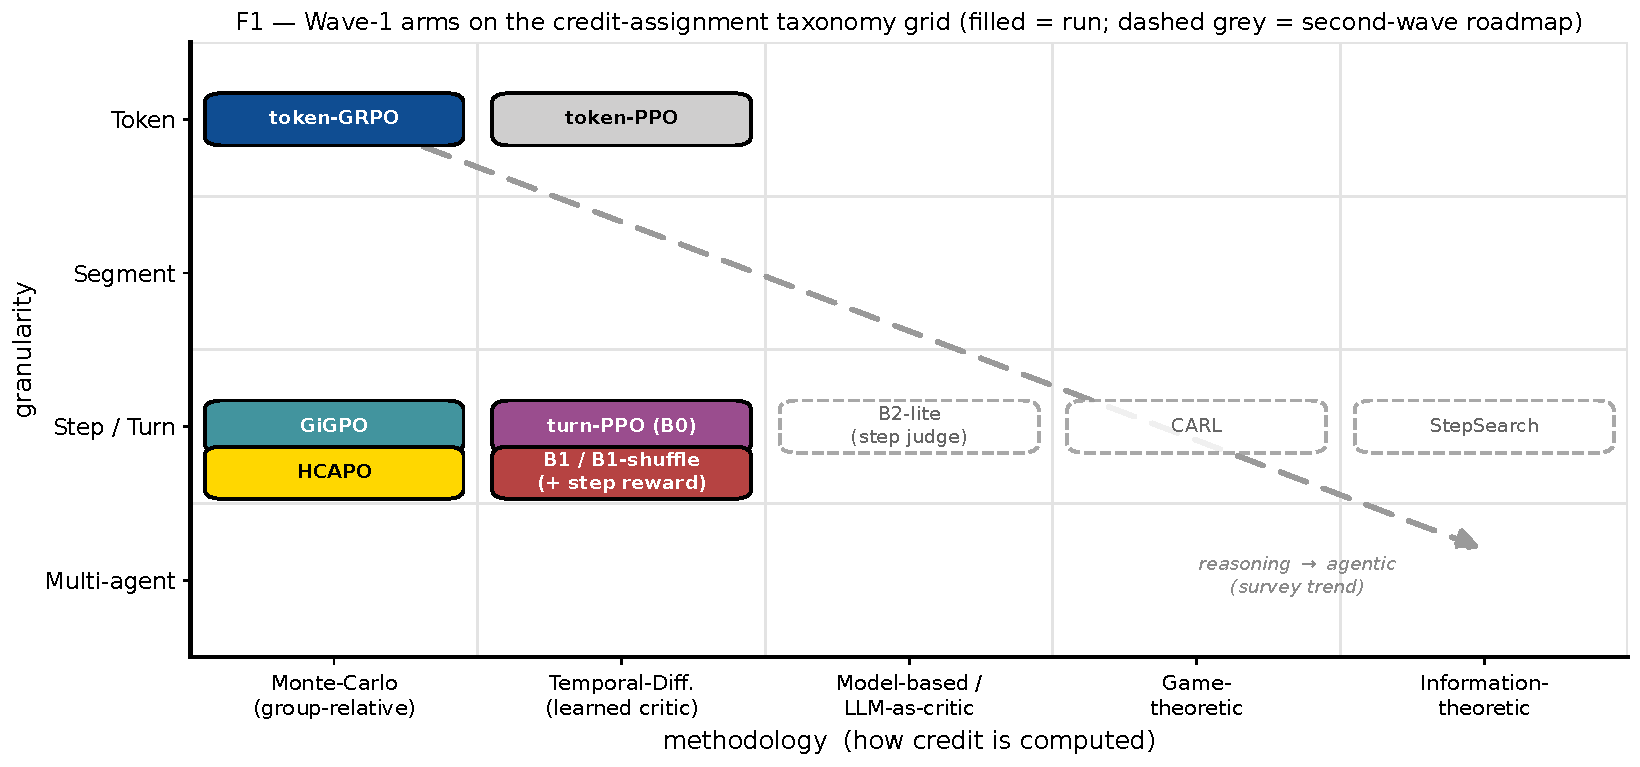
\includegraphics[width=\textwidth]{fig_taxonomy.pdf}
\caption{\textbf{F1 --- the Wave-1 arms on the survey's credit-assignment taxonomy grid}
(granularity $\times$ methodology, arXiv~2604.09459 Fig.~2). Filled chips are run in Wave~1,
coloured by family; dashed grey chips are the second-wave roadmap (B2-lite step judge, CARL,
StepSearch). The study populates the Monte-Carlo (group-relative) and Temporal-Difference
(learned-critic) columns at Token and Step/Turn granularity --- exactly the contrast H1--H3
target.}
\label{fig:tax}
\end{figure}

\section{Experimental design}

\textbf{Task.} Search-R1 protocol: the agent answers open-domain questions by interleaving
\texttt{<think>} reasoning with either \texttt{<search>query</search>} or a final
\texttt{<answer>...</answer>}, for up to 4 turns (main) or 8 (stress test). Retrieval is dense e5
over the 2018 Wikipedia dump (wiki-18, 61\,GB FAISS index), top-3 passages/query, served by a
co-located retrieval server. \textbf{Training data:} the standard Search-R1 mixture (NQ~+~HotpotQA
train, HF \texttt{PeterJinGo/nq\_hotpotqa\_train}), versioned preprocessing. \textbf{Validation}
during training uses a fixed stratified 2{,}048-question subset (\texttt{val\_2048}, greedy, every
25 steps); final evaluation is the full paper-protocol test set (\textbf{51{,}713 questions, 7
datasets}, greedy EM). \textbf{Reward:} rule-based EM on the final answer plus a small
invalid-action penalty --- no learned reward model in the core tier, so the only intermediate
signal is the one we inject and control. \textbf{Model:} Qwen3-1.7B (thinking mode, 2{,}048-token
responses, 4{,}096-token prompts), identical across arms; batch 256, group 5, 500 steps, matched
LR/KL. A pre-registered feasibility gate on the \emph{untrained} model (macro-EM floor $\geq$0.03,
valid-action $\geq$90\%, search-invocation $\geq$50\%, within-group reward variance) passed at
1.7B, so the fleet stayed at this scale.

\begin{table}[h]
\centering\small
\begin{tabular}{lllp{5.7cm}}
\toprule
Arm & Estimator & Critic & Where the ``reward model'' lives \\
\midrule
\arm{token-PPO}   & GAE (token)      & yes & implicit: token-level value network \\
\arm{turn-PPO/B0} & GAE (turn)       & yes & implicit: turn-level value network \\
\arm{token-GRPO}  & GRPO             & no  & implicit: group-relative outcome baseline \\
\arm{GiGPO}       & GiGPO            & no  & implicit: episode + anchor-state grouped baselines \\
\arm{HCAPO}       & HCAPO            & no  & implicit: hindsight-conditioned per-turn advantage amplifier \\
\arm{B1}          & GAE (turn) + step reward & yes & \textbf{explicit}: privileged answer-exposure signal, $+0.2$ the first turn whose retrieved passages contain the gold answer \\
\arm{B1-shuffle}  & GAE (turn) + shuffled step reward & yes & \textbf{explicit, contentless}: B1's rewards re-assigned to another non-terminal search turn --- matched count/magnitude, destroyed timing \\
\bottomrule
\end{tabular}
\caption{The seven core arms. B1 is deliberately \emph{privileged and verifiable} (it peeks at the
gold answer) --- an upper-bound proxy for a perfect progress reward, free of judge noise. The
shuffled control isolates information content from reward density.}
\end{table}

\textbf{Pre-registered decision rules.} Primary comparison = fixed-budget \emph{final} checkpoint
(@500); sample-efficiency = validation AUC; best-val checkpoint reported but never the headline.
RQ3 is judged on per-seed final-EM deltas with seed ranges (2--3 seeds/arm) plus a paired
per-dataset breakdown with the multi-hop subgroup as the mechanism readout. \textbf{Interpretation
grid:} B1 $>$ shuffle $\approx$ B0 $\Rightarrow$ content matters; B1 $\approx$ shuffle $>$ B0
$\Rightarrow$ density effect; all $\approx$ $\Rightarrow$ this signal does not help at this
horizon. The \texttt{shuffle\_active\_frac} (fraction of B1-positive trajectories with $\geq$2
eligible search turns) is reported beside any B1-vs-shuffle claim; a Wave-1 value below $\sim$30\%
promotes the 8-turn stress test from optional to \emph{required} (it did --- \S\ref{sec:rq3}).

\section{Results}

All 17 runs reached the 500-step budget. Table~\ref{tab:finals} and Fig.~\ref{fig:bars} give the
pre-registered primary comparison; Fig.~\ref{fig:curves} the learning curves.

\begin{table}[h]
\centering\small
\begin{tabular}{lll r r r l}
\toprule
Arm & Credit family & Gran. & Seeds & Mean & Range & Clip health \\
\midrule
\arm{GiGPO}       & critic-free group-rel. & turn  & 2 & \textbf{0.397} & 0.396--0.398 & clean ($\approx$0) \\
\arm{token-GRPO}  & critic-free group-rel. & traj. & 2 & \textbf{0.394} & 0.389--0.399 & clean ($\approx$0) \\
\arm{HCAPO}       & critic-free amplifier  & turn  & 1 & 0.357 & --- & \textbf{collapse, clip 0.754} \\
\arm{B1-shuffle}  & critic + shuffled step & turn  & 3 & 0.353 & 0.340--0.363 & clean \\
\arm{B1}          & critic + privileged step & turn & 3 & 0.347 & 0.318--0.372 & drift; s1 collapsed \\
\arm{turn-PPO/B0} & critic                 & turn  & 3 & 0.332 & 0.324--0.343 & drift, all seeds \\
\arm{token-PPO}   & critic                 & token & 1 & 0.315 & --- & persistent drift \\
\midrule
\arm{B0}, 8-turn  & critic                 & turn  & 1 & 0.368 & --- & clean-ish (0.037) \\
\arm{B1}, 8-turn  & critic + step          & turn  & 1 & 0.343 & --- & drift (0.15$\to$0.27) \\
\bottomrule
\end{tabular}
\caption{Final val-2048 macro-EM at the fixed-budget checkpoint (@500), the pre-registered primary
metric. Untrained baseline 0.2246. Range = min--max across seeds. ``Clip'' = response-length
truncation ratio (fraction of turn responses hitting the 2{,}048-token cap; healthy $\approx$0).
Backing data: \texttt{assets/figs/finals.csv}, one row per seeded run, regenerated from the launch
logs.}
\label{tab:finals}
\end{table}

\begin{figure}[t]
\centering
\includegraphics[width=0.94\textwidth]{fig_final_bars.pdf}
\caption{\textbf{Headline: fixed-budget final val macro-EM, 4-turn arms.} Dots are individual
seeds, whiskers min--max. Outcome-only group-relative methods (GiGPO, token-GRPO; cool colours)
lead by 4--6 points over every critic and step-reward arm --- \emph{without} a critic network.
HCAPO reaches a middling 0.357 but only via a truncation collapse (clip$\to$0.75, flagged;
Fig.~\ref{fig:trip}). The explicit progress reward (B1) does not beat its shuffled placebo
(B1-shuffle).}
\label{fig:bars}
\end{figure}

\begin{figure}[t]
\centering
\includegraphics[width=\textwidth]{fig_learning_curves.pdf}
\caption{Validation macro-EM (val\_2048, greedy, every 25 steps); band = seed min--max.
\textbf{(a)} Granularity \& outcome-only CA: GiGPO and token-GRPO climb steadily to $\approx$0.40;
the critic PPO arms plateau near 0.33; token-PPO is weakest; HCAPO (amber) plateaus at 0.35 as it
destabilises. \textbf{(b)} The RQ3 triad at 3 seeds/arm: the three conditions are statistically
inseparable throughout, with B1-shuffle (control) tracking at or above B1 (privileged content).
\textbf{(c)} Horizon stress: the 8-turn budget lifts the sparse B0 baseline above its 4-turn self,
but 8-turn B1 sits below 8-turn B0.}
\label{fig:curves}
\end{figure}

\subsection{Finding 1 --- outcome-only group-relative CA wins, and costs less}

GiGPO (0.397) and token-GRPO (0.394) beat every critic-based and step-reward arm by 4--6 points
(Table~\ref{tab:finals}, Fig.~\ref{fig:bars}), solidified at two seeds each with clean clip health
throughout. Both use \emph{no} critic network, and on wall-clock they were the \emph{cheapest}
arms ($\approx$29--30\,h vs.\ $\approx$33--37\,h for the critic arms on the same 8$\times$H100
worker; \S\ref{sec:compute}) --- the critic is pure overhead here that also hurts accuracy and
stability. H1 (granularity) holds directionally: turn-PPO (0.332) $\geq$ token-PPO (0.315) at
matched config, though both trail the critic-free arms. This is the study's cleanest positive
result and directly answers H2 on accuracy; Finding~4 supplies the mechanism.

\subsection{Finding 2 (RQ3) --- privileged content adds nothing over its shuffle}
\label{sec:rq3}

At three seeds per arm the pre-registered comparison reads
\[
\text{B1-shuffle } 0.353 \;\geq\; \text{B1 } 0.347 \;>\; \text{B0 } 0.332,
\]
i.e.\ both dense-reward arms beat sparse B0 by a small margin, but the \emph{shuffled placebo
matches or exceeds the real privileged content} (Fig.~\ref{fig:rq3}). Per the pre-registered
interpretation rule (``B1 $\approx$ B1-shuffle $>$ B0 $\Rightarrow$ density/optimization effect,
not supervision''), this is \textbf{a reward-density effect, not progress-content supervision}.
The dynamics corroborate the reading (Fig.~\ref{fig:dyn}): the contentless shuffle arm
\emph{saturates the turn budget} (final avg.\ 4.00 turns) --- a dense reward on search turns
teaches ``search \emph{more}'', not ``search \emph{better}'' --- yet loses no accuracy and stays
clip-clean, whereas B1 answers in fewer turns (avg.\ 3.00) but destabilises (clip 0.19).
B1's seed variance is wide (0.318--0.372); the shuffle is tighter (0.340--0.363), so the control
is also the more reliable arm.

\textbf{On the validity of the 4-turn control.} \texttt{shuffle\_active\_frac} was 0.035 on the
\emph{base}-model distribution --- far below the 0.30 rule --- which fired the pre-registered
plan~B and \emph{promoted the 8-turn stress test to required} (Finding~5). But during RL the
metric \emph{inverted}: as the policy learned to issue more searches, active\_frac rose past 0.30
to $\approx$0.97--1.0 on the training batches that produced the finals. So the 4-turn control was
in fact \emph{fully discriminating} for the reported comparison --- the density reading does not
hinge on a degenerate control.

\begin{figure}[t]
\centering
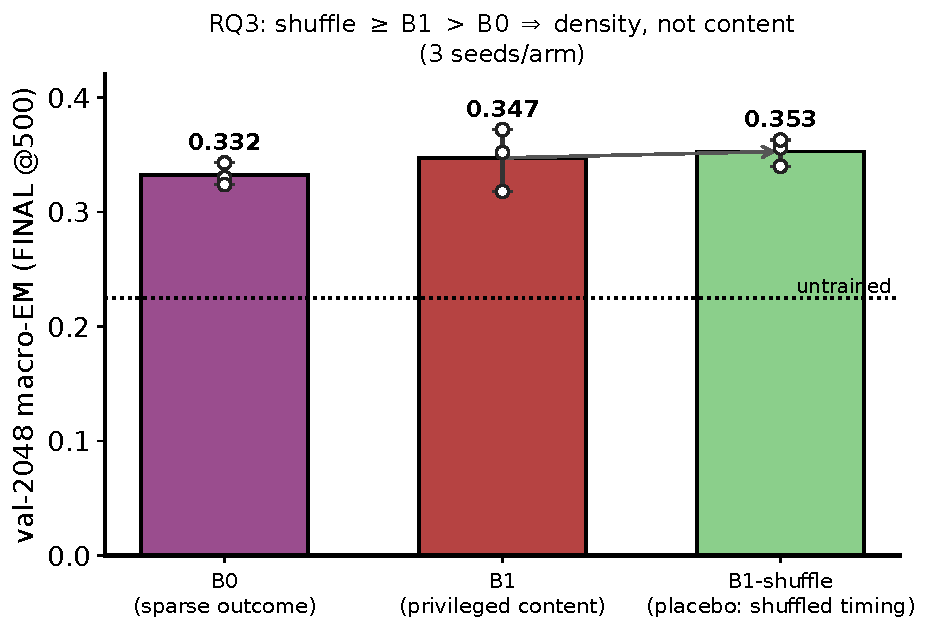
\includegraphics[width=0.49\textwidth]{fig_rq3_density.pdf}\hfill
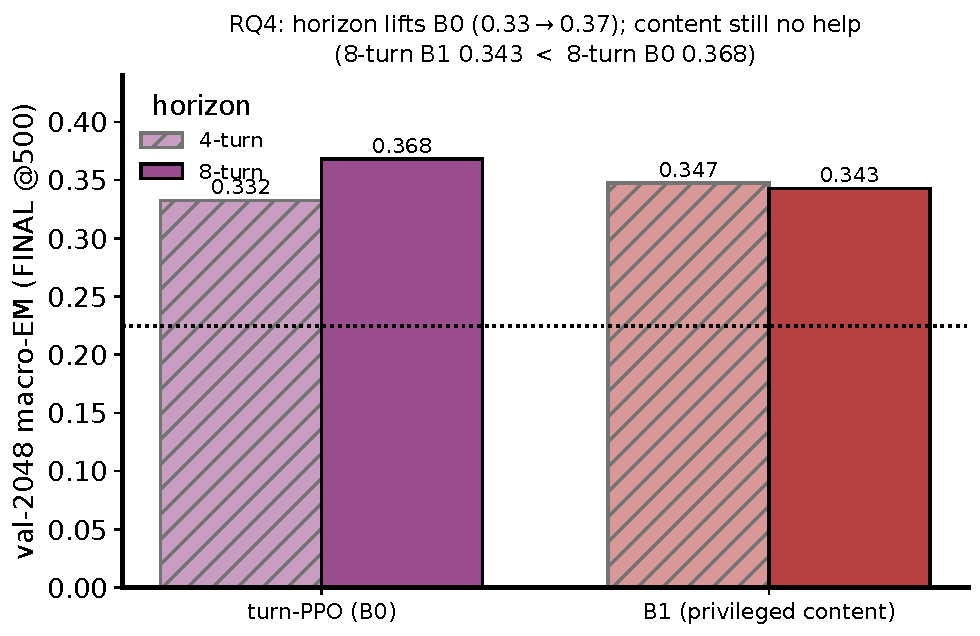
\includegraphics[width=0.49\textwidth]{fig_rq4_horizon.pdf}
\caption{\textbf{Left (RQ3, Finding 2):} the privileged-content arm (B1) does not beat its
density-matched placebo (B1-shuffle); both edge out sparse B0. 3 seeds/arm, dots per seed.
\textbf{Right (RQ4, Finding 5):} the 8-turn horizon lifts the sparse baseline
($0.332\to0.368$), but the privileged content still does not help (8-turn B1 $0.343 <$ 8-turn
B0 $0.368$); the step-200 early hint (B1 0.358 $>$ B0 0.338) did not hold to the final.}
\label{fig:rq3}
\end{figure}

\begin{figure}[t]
\centering
\includegraphics[width=\textwidth]{fig_reward_turns.pdf}
\caption{Training dynamics (seed-0 arms). \textbf{(a)} Mean episode reward; B1/B1-shuffle sit
higher by construction (the $+0.2$ step bonus). \textbf{(b)} Average turns per trajectory. Note
B1-shuffle saturating the 4-turn budget and HCAPO's high turn usage; dashed = 8-turn arms, which
use only $\approx$4.4 of 8 available turns.}
\label{fig:dyn}
\end{figure}

\subsection{Finding 3 --- truncation instability tracks aggressive per-turn credit}

The single most reproducible \emph{mechanistic} result is a late-training response-truncation
runaway (Fig.~\ref{fig:trip}). It scales with how aggressively an arm concentrates credit on
individual turns: HCAPO --- a critic-free \emph{per-turn advantage amplifier} --- blows up
completely (clip $\to0.754$, generating over-long per-turn responses that hit the 2{,}048-token
cap 75\% of the time) while its accuracy merely plateaus at $\approx$0.35, so the ``collapse''
buys nothing; every critic arm drifts upward (token-PPO 0.10, B0 0.14, B1 0.19, 8-turn B1 0.27);
and everything group-relative-and-flat (GiGPO, token-GRPO, and the shuffled B1) stays at
clip $\approx$0 throughout. This reframes late-training length instability as a
\emph{first-class cost} of aggressive per-turn credit weighting --- a stability, not just
accuracy, axis on which the outcome-only group-relative methods dominate. It is also the mechanism
behind B1's wide seed variance (its s1 collapsed to 0.318).

\begin{figure}[t]
\centering
\includegraphics[width=\textwidth]{fig_tripwire.pdf}
\caption{\textbf{Finding 3 --- the truncation tripwire.} \textbf{(a)} Response-length clip ratio
over training (must fall to $\approx$0). HCAPO's per-turn amplifier runs away to 0.75; the critic
arms drift up; group-relative-and-flat arms (GiGPO, GRPO, B1-shuffle) stay clean.
\textbf{(b)} HCAPO in detail: clip climbs to 0.75 while val macro-EM plateaus at $\approx$0.35 ---
the length runaway yields no accuracy, it is pure degeneration.}
\label{fig:trip}
\end{figure}

\subsection{Finding 4 (F8a) --- the critic assigns credit uncorrelated with true progress}

To test H2 quantitatively --- does a method assign \emph{correct} intermediate credit, not just
train a better policy? --- we ran the pre-registered credit-alignment diagnostic on the turn
critic. For logged trajectories at fixed B0 checkpoints we estimated each prefix's outcome-only
Monte-Carlo continuation value $\hat V(s_t)=\frac1K\sum_k R(\tau_k\mid s_t)$ by resuming from the
prefix under the \emph{same} checkpoint (K=8), giving the martingale-increment
$\Delta\hat V_t=\hat V(s_{t+1})-\hat V(s_t)$ --- the credit an ideal process reward would assign.
We compared it to the critic's own one-step delta $A_t=V_\phi(s_{t+1})-V_\phi(s_t)$.
Across all four checkpoints the pooled Spearman correlation is indistinguishable from zero
($\rho\in[-0.02,\,0.11]$, bootstrap 95\% CIs spanning 0; sign agreement $\approx$0.15;
Fig.~\ref{fig:f8a}), so \textbf{0 of 3 gate checkpoints passed the pre-registered unlock threshold}
($\rho>0.2$ with CI excluding 0) and the planned $\lambda$-bootstrapping sweep was
\textbf{dropped and is reported here as a negative}. The turn critic functions only as a weak
trajectory-level baseline (value explained-variance $\approx$0.28), \emph{not} as a per-turn
reward model. This is the mechanism behind Finding~1: bootstrapping through a critic that carries
essentially no per-turn progress information ($\lambda<1$) has no basis here, which is exactly why
the critic arms trail the flat group-relative baselines.

\begin{figure}[t]
\centering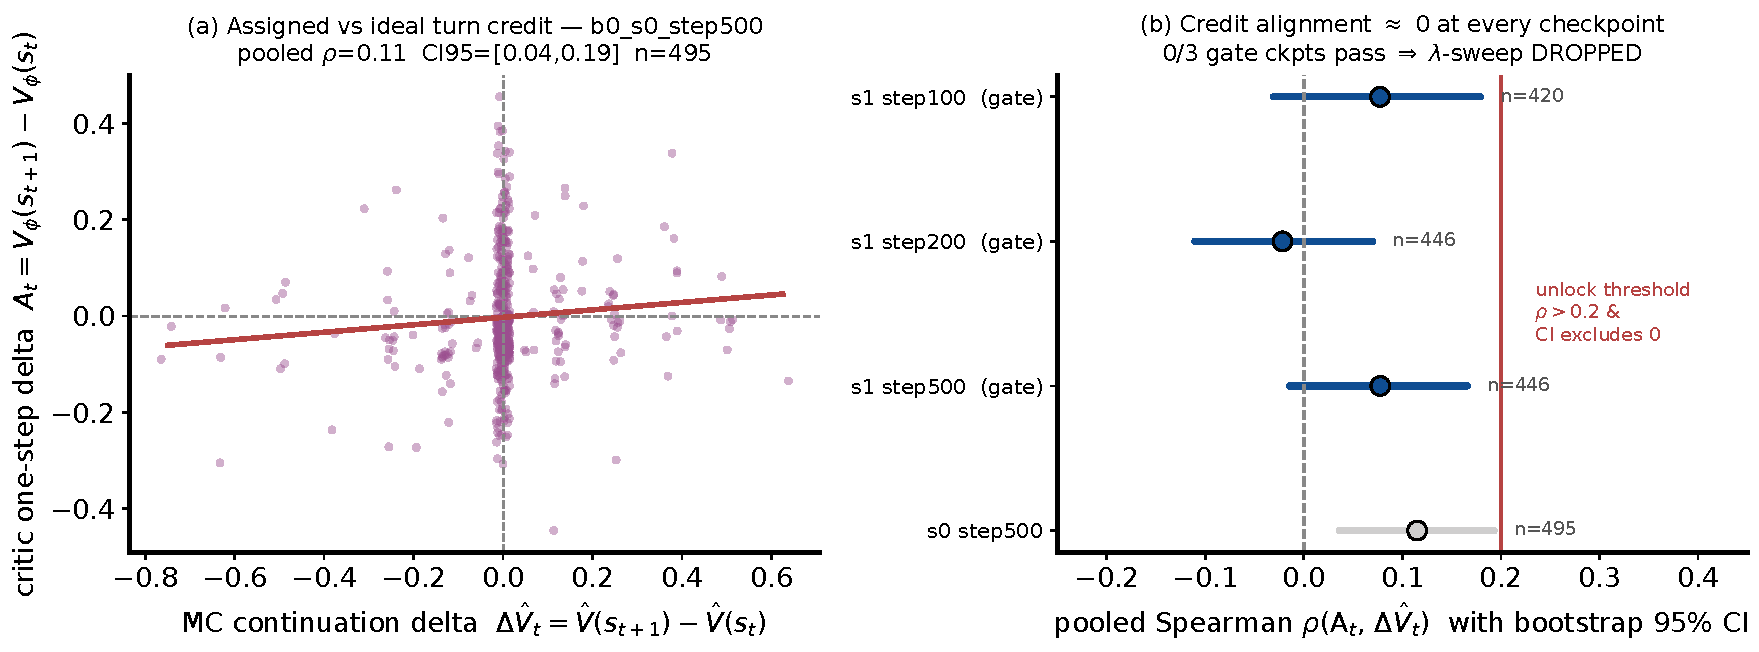
\includegraphics[width=\textwidth]{fig_f8a_credit_alignment.pdf}
\caption{\textbf{Finding 4 --- credit alignment $\approx0$.} \textbf{(a)} Critic one-step delta
$A_t$ vs.\ the Monte-Carlo continuation delta $\Delta\hat V_t$ (the ``ideal'' credit), pooled over
turn-pairs at the best-populated checkpoint (n=495); the least-squares fit is nearly flat.
\textbf{(b)} Pooled Spearman with bootstrap 95\% CI at every diagnostic checkpoint; none clears the
$\rho>0.2$ unlock threshold, so the $\lambda$-sweep is dropped as a pre-registered negative.}
\label{fig:f8a}
\end{figure}

\subsection{Finding 5 (RQ4) --- horizon lifts the baseline, content still does not help}

The 8-turn stress test (promoted to required by the base-distribution active\_frac; \S\ref{sec:rq3})
gives a decisive horizon readout (Fig.~\ref{fig:rq3}, right). The longer budget \emph{lifts the
sparse baseline itself}: 8-turn B0 = 0.368 $>$ 4-turn B0 mean 0.332. But the privileged progress
content still does not help: \textbf{8-turn B1 = 0.343 $<$ 8-turn B0 = 0.368}, and the step-200
early hint (B1 0.358 $>$ B0 0.338) did \emph{not} hold to the final --- B1's added reward density
drove clip drift ($0.15\to0.27$) and a mild degradation (peak 0.362 $\to$ 0.343). So the marginal
value of this progress supervision does \emph{not} grow with horizon; it is $\leq$0 here,
consistent with the 4-turn density reading. \emph{Caveat (pre-logged):} no 8-turn shuffle control
was run, so 8-turn B1 $<$ B0 cannot fully separate content from density --- but the direction (no
benefit, mild harm) is unambiguous and matches the fully-controlled 4-turn result.

\subsection{Full-set evaluation (proxy validation) and the multi-hop subgroup}

One arm has completed the full 51{,}713-question paper-protocol evaluation so far --- token-GRPO
seed~0 at its final checkpoint (Table~\ref{tab:fullset}). Its full-set macro-EM is
\textbf{0.3951} (micro 0.4433), within $\approx$0.006 of its val\_2048 proxy (0.389) ---
\textbf{validating the fixed subset as the training-time metric}. The pre-registered single- vs
multi-hop split is stark: 0.499 single-hop vs.\ 0.317 multi-hop, with MuSiQue (the hardest
4-hop set) at 0.142. Turn usage rises with difficulty (avg.\ 3.1 single-hop $\to$ 3.6 MuSiQue)
and \emph{no} trajectory was left unterminated (0\% truncation on the answer turn). Full-set evals
of the remaining final checkpoints are the immediate Wave-4 GPU task; they will populate the
per-dataset $\Delta$EM breakdown for every arm.

\begin{table}[h]
\centering\small
\begin{tabular}{l l r r r r}
\toprule
Dataset & Subgroup & $n$ & EM & avg.\ turns & unterm. \\
\midrule
NQ              & single-hop & 3{,}610  & 0.445 & 3.15 & 0\% \\
TriviaQA        & single-hop & 11{,}313 & 0.602 & 3.12 & 0\% \\
PopQA           & single-hop & 14{,}267 & 0.450 & 3.14 & 0\% \\
HotpotQA        & multi-hop  & 7{,}405  & 0.396 & 3.31 & 0\% \\
2WikiMultihopQA & multi-hop  & 12{,}576 & 0.378 & 3.46 & 0\% \\
MuSiQue         & multi-hop  & 2{,}417  & 0.142 & 3.61 & 0\% \\
Bamboogle       & multi-hop  & 125      & 0.352 & 3.58 & 0\% \\
\midrule
\multicolumn{2}{l}{\textbf{macro / micro}} & 51{,}713 & \textbf{0.395} / 0.443 & 3.3 & 0\% \\
\multicolumn{2}{l}{single-hop / multi-hop macro} & & 0.499 / 0.317 & & \\
\bottomrule
\end{tabular}
\caption{Full-set paper-protocol EM for token-GRPO s0 (final checkpoint). Base untrained model on
the same protocol: 0.301 single-hop / 0.167 multi-hop macro. Source:
\texttt{eval\_full/wave0\_grpo\_s0\_final/paper\_table.json}.}
\label{tab:fullset}
\end{table}

\section{Compute accounting}
\label{sec:compute}

Closing the survey's \#1 reporting gap (0/41 CA papers report GPU-hours): the 17 completed
500-step training runs used \textbf{$\approx$4.7k GPU-hours} (8$\times$H100 each; per-run
wall-clock measured launch-to-completion on clean runs --- $\approx$29--30\,h for a 4-turn
critic-free run, $\approx$33--37\,h for a 4-turn critic run, $\approx$45\,h for an 8-turn run,
$\times$8 GPUs). Including the failed-attempt reruns (early-Wave OOM cycles resolved by a
micro-batch protocol fix), the F8a diagnostic worker sessions, the full-set eval, and the Wave-0
feasibility/toy-gate runs, the project total is \textbf{$\approx$5.5k GPU-hours}. \textbf{CA
overhead by arm} (survey item \#12): critic-free group-relative CA has \emph{negative} overhead
--- it removes the critic's forward/backward, running $\approx$15--20\% faster per step than PPO;
HCAPO adds a hindsight relabelling pass (cheap in compute, expensive in stability); B1/B1-shuffle
add only an env-side gold-answer string match per turn (and a seeded driver-side reassignment for
the shuffle). The expensive add-on is the offline F8a diagnostic (prefix-resume + K continuations
per prefix), one worker for a few hours.

\section{Discussion}

The five findings converge on one thesis: \textbf{for this multi-turn search task, outcome-only
group-relative credit assignment is the right default} --- it is the most accurate, the most
stable, and the cheapest, and explicit privileged progress supervision adds no value that its own
density-matched shuffle does not already provide, at either 4 or 8 turns. The critic-based
alternative is not merely weaker but \emph{mechanistically} deficient: its per-turn value deltas
carry essentially no true-progress information (Finding~4), which explains both its accuracy gap
and --- through aggressive per-turn credit weighting --- its truncation instability (Finding~3).

\textbf{Scope of the claim (from the pre-registration, not hedging after the fact).} This is
evidence about \emph{this} privileged answer-exposure signal at \emph{this} horizon on \emph{this}
task; it is \emph{not} a claim that progress reward models are useless in general. B1 is a
verifiable upper-bound proxy free of judge noise --- that it fails to beat its shuffle is a strong
negative for the ``dense progress signal helps'' hypothesis in this regime, but a genuinely
informative learned PRM on a longer-horizon task with sparser reward could still help; that is the
B2/CARL second wave. \textbf{Open items:} full-set evals of the remaining final checkpoints (the
per-dataset $\Delta$EM breakdown; Wave-4 GPU); HCAPO/token-PPO second seeds; and the second-wave
methods (CARL, B2-lite step judge, StepSearch) each behind their own gate.

\clearpage
\appendix

\section{Reporting checklist (survey Table 11) --- filled}

Per the project standard, every report fills the CA survey's reporting checklist
(\texttt{docs/CREDIT\_ASSIGNMENT\_CHECKLIST.md}). This study was \emph{designed} to close the
survey's three systemic gaps (GPU-hours 0/41; compute-controlled baseline 0/41; variance 2/41).

\begin{table}[h]
\centering\footnotesize
\begin{tabular}{c l l p{7.6cm}}
\toprule
\# & Category & Priority & How this study reports it \\
\midrule
1  & Model \& Data & Req. & Qwen3-1.7B, thinking mode, HF revision pinned in configs \\
2  & Model \& Data & Req. & Search-R1 NQ+HotpotQA train; versioned preprocessing; 51{,}713-q / 7-dataset test \\
3  & CA Method & Req. & granularity per arm (token / turn / trajectory), Table~\ref{tab:finals} + F1 \\
4  & CA Method & Req. & methodology family per arm (MC group-relative / TD critic), F1 grid \\
5  & Baselines & Req. & episode-level token-PPO \emph{and} token-GRPO, identical base model \\
6  & Baselines & Req. & \textbf{compute-controlled}: B1-shuffle is density-matched; iso-worker critic-vs-critic-free wall-clock reported \\
7  & Baselines & Rec. & CA-component isolation: B1 vs B1-shuffle (content vs density); $\lambda$-gate on the critic \\
8  & Evaluation & Req. & val\_2048 (train-time) + full 51{,}713-q paper test, exact splits named \\
9  & Evaluation & Req. & macro/micro EM, exact match on final answer, defined in \S3 \\
10 & Evaluation & Rec. & \textbf{variance}: 2--3 seeds/arm, min--max ranges in Table~\ref{tab:finals} \\
11 & Compute & Req. & \textbf{GPU-hours}: $\approx$4.7k training / $\approx$5.5k total, \S\ref{sec:compute} \\
12 & Compute & Rec. & CA overhead per arm (critic-free negative; HCAPO hindsight; diagnostic cost), \S\ref{sec:compute} \\
13 & Trajectory & Req. & avg.\ turns per arm (Table~\ref{tab:finals} data; 2.5--4.0), full-set avg.\ 3.3 \\
14 & Trajectory & Rec. & turns min/median/max per dataset, Table~\ref{tab:fullset} + \texttt{paper\_table.json} \\
\bottomrule
\end{tabular}
\end{table}

\noindent\textbf{Table-12 scorecard (this study vs.\ the survey's three exemplars).}
\chk\ reported, \prt\ partial, \non\ not reported.

\begin{table}[h]
\centering\footnotesize
\begin{tabular}{l l c c c c}
\toprule
Category & Item & HICRA & GiGPO & M-GRPO & \textbf{This study} \\
\midrule
Model      & Base model name/size            & \chk & \chk & \chk & \chk \\
Model      & Training data source/size       & \prt & \prt & \non & \chk \\
CA Method  & Credit granularity              & \chk & \chk & \chk & \chk \\
CA Method  & Methodology family              & \chk & \chk & \chk & \chk \\
Baselines  & Episode-level baseline (same model) & \chk & \chk & \chk & \chk \\
Baselines  & \textbf{Compute-controlled baseline} & \non & \non & \non & \chk \\
Baselines  & CA-component ablation            & \chk & \prt & \non & \chk \\
Evaluation & Benchmark names + splits         & \chk & \chk & \prt & \chk \\
Evaluation & \textbf{Variance / CIs}          & \prt & \non & \non & \chk \\
Compute    & \textbf{Total GPU-hours}         & \non & \non & \non & \chk \\
Compute    & CA-specific overhead             & \prt & \prt & \non & \chk \\
Trajectory & Avg trajectory length            & \prt & \chk & \non & \chk \\
\bottomrule
\end{tabular}
\caption{The study reports all three of the survey's systemic gaps (bold rows): compute-controlled
baseline, variance across seeds, and total GPU-hours.}
\end{table}

\section{Annotated example trajectory and per-method credit}

A trained token-GRPO trajectory from the full-set eval (traj \texttt{a1c80bb0}, HotpotQA, 3 turns,
EM~=~1; reconstructed from the logged rollout). Turn-by-turn text with the credit each family
\emph{would} assign, so the credit assignment is inspectable:

\begin{Verbatim}[fontsize=\footnotesize,frame=single]
QUESTION: Are Scott Derrickson and Ed Wood of the same nationality?

TURN 0  <think>I need each director's nationality. Start with Ed Wood.</think>
        <search>Ed Wood nationality</search>
        <information>Doc: Edward D. Wood Jr. was an American filmmaker ...</information>

TURN 1  <think>Ed Wood is American. Now Scott Derrickson.</think>
        <search>Scott Derrickson nationality</search>
        <information>Doc: Scott Derrickson is an American director (Doctor Strange) ...</information>

TURN 2  <think>Both are American, so the answer is yes.</think>
        <answer>yes</answer>                           --> outcome reward 1.0
\end{Verbatim}

\noindent\textbf{What each arm assigns to this trajectory (turns 0,1,2):}
\begin{itemize}\itemsep1pt
  \item \arm{token-GRPO}: one trajectory-level advantage (group-relative to the batch), broadcast
  uniformly to every response token of all three turns --- no per-turn distinction.
  \item \arm{GiGPO}: a group-relative advantage \emph{per turn}, comparing each turn against an
  anchor group of same-state siblings --- turns 0 and 1 (both answer-advancing searches) score
  positively.
  \item \arm{turn-PPO/B0}: the critic's per-turn value delta $A_t$ --- which Finding~4 shows is
  essentially uncorrelated with the true continuation-value progress of turns 0$\to$1$\to$2.
  \item \arm{B1}: B0's credit \emph{plus} $+0.2$ on turn~0 (the first retrieval containing the
  gold string ``American''), first-hit-only.
  \item \arm{B1-shuffle}: the same $+0.2$ re-assigned to another eligible non-terminal search turn
  (here turn~1) --- matched magnitude, destroyed timing. Findings 2/5: this changes nothing.
\end{itemize}

\vspace{0.4em}
\noindent\textbf{Reproducibility.} Figures + finals: \texttt{assets/extract\_metrics.py}
(launch-log $\to$ per-run CSV) $\to$ \texttt{assets/build\_figures.py} +
\texttt{build\_f8a.py} + \texttt{build\_taxonomy.py} (see \texttt{assets/figs/README.md} for the
per-figure data map). Training logs, the worker ledger (GPU-hours), and the append-only decision
log live in the project repository (\texttt{Agentic-RL-CA}, branch \texttt{agentic-rl-ca});
pre-registration in \texttt{docs/plan.md}; the credit-alignment diagnostic in
\texttt{credit\_assignment/\{diagnostic,lambda\_gate\}.py}.

\end{document}
